Given,
\begin{align}
\vec{P} = \myvec{7\\6} \quad
\vec{Q} = \myvec{3\\4}    
\end{align}
A vector on  the  X-axis  $\vec{X}$  is  equidistant  to  both  $\vec{P}$  and $\vec{Q}$.
\begin{align}
i.e. \ \vec{X} = \frac{{\vec{P}+\vec{Q}}}{2}    
\end{align}
Need to find  k. 
Let $\vec{X}$ = k\myvec{1\\0}  be  the  vector  on  the  X-axis.
\begin{align}
\implies \myvec{1 & 0}\vec{X} = k \\
\implies \vec{X} = \frac{\myvec{7\\6}+\myvec{3\\4}}{2} \\
\implies \vec{X} = \myvec{5\\5} \\
\implies \myvec{1 & 0}\vec{X} = \myvec{1 & 0}\myvec{5\\5} \\ 
\end{align}
Therefore, k = 5 \ i.e. $\vec{X}$ = \myvec{5\\0}
See Fig.     \ref{Fig.1solutions/point_vector/22/}

\begin{figure}[!htb]
    \centering
    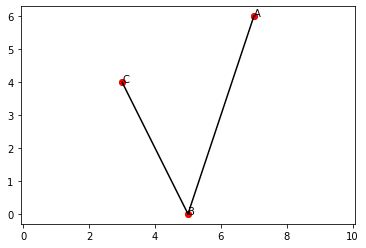
\includegraphics[width=\columnwidth]{./solutions/point_vector/22/Assignment1.png}
    \caption{Plot representing the Points}
    \label{Fig.1solutions/point_vector/22/}
\end{figure}
